\section{Тестирование}\label{sec:evaluation}
Для тестирования моделей, предложенных в главе \ref{sec:model}, применялись датасеты для трех языков, использовавшиеся в недавних работах других исследователей: решения задач GCJ для Python \cite{Alsulami2017} и C++ \cite{Caliskan2015}, набор из 40 проектов с открытым исходным кодом для Java \cite{Yang2017}. Эти три датасета представляют собой наиболее актуальные результаты для каждого из языков среди работ, использовавших данные находящиеся в открытом доступе. Результаты сравнения приведены в таблице \ref{tab:results-comparison}. Помимо тестирования на указанных датасетах были проведены эксперименты с данными проекта IntelliJ IDEA, более подробно описанными в главе \ref{sec:data}.

\subsection{Сравнение с предыдущими работами}

\subsubsection{Java}
Датасет для Java состоит из 40 проектов, написанных разными авторами. Он включает в себя 3021 файл, число файлов в проектах варьируется от 11 до 712 с медианой 54. Из-за значительного различия в числе доступных примеров между разработчиками датасет является несбалансированным. Поскольку в среднем число примеров не превышает сотни, из двух предложенных в этой работе моделей лучшие результаты показывает случайный лес, специально созданный для работы в условиях небольшого количества данных.

Сравнение производилось с лучшим на данный момент решением, использовавшим этот набор данных \cite{Yang2017}. Для получения сравнимых результатов применяется такое же разбиение данных, как и в вышеуказанной работе. Все файлы разбиваются на 10 частей, или фолдов, в каждую из которых попадает одинаковое количество примеров от каждого из авторов. Например, от разработчика с 31 файлом в одной части окажется четыре файла, а в остальных по три. Затем проводится 10 экспериментов, в каждом из которых одна часть представляет тестовую выборку, а остальные — тренировочную. По выборке, состоящей из результатов экспериментов, вычисляется выборочное среднее и дисперсия, которые затем сравниваются с результатами предыдущей работы.

Для применения случайного леса требуется подобрать оптимальные гиперпараметры, к которым относится число деревьев и количество используемых факторов. Для подбора оптимальных гиперпараметров была проведена серия экспериментов с разным количеством деревьев и разным количеством факторов. Средняя точность и отклонение, полученные в результате кроссвалидации, в зависимости от варьируемых параметров приведены на Рис. \ref{fig:hyper-trees} для числа деревьев и на Рис. \ref{fig:hyper-factors} для числа факторов. Точность при оптимальном выборе параметров значительно превосходит результаты предыдущей работы \cite{Yang2017}: 97\% против 91.1\%.


\begin{figure}[ht]
    \centering
       \begin{subfigure}{0.49\linewidth}
       \centering
       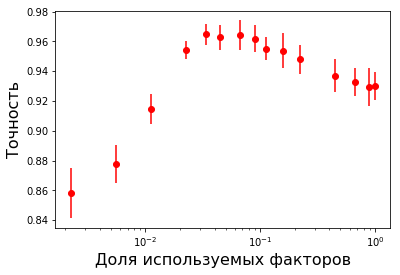
\includegraphics[width=\linewidth]{images/factors.png}
       \caption{}
       \label{fig:hyper-factors} 
    \end{subfigure}
    % \\[\baselineskip]
    \hfill
    \begin{subfigure}{0.49\linewidth}
       \centering
       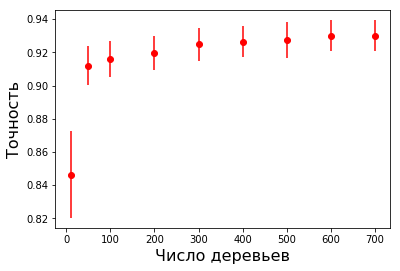
\includegraphics[width=\linewidth]{images/trees.png}
       \caption{}
       \label{fig:hyper-trees}
    \end{subfigure}
    \centering
    \caption{Зависмость точности и стандартного отклонения для датасета на языке Java от (a) доли используемых факторов; (b) числа деревьев.}
    \end{figure}

Использование нейросетевой модели показало точность 86\%, что хуже чем результаты случайного леса и нейросети, обученной при помощи PSO \cite{Yang2017}. При этом результаты оказались выше, чем у той же нейросети, обученной при помощи SGD. Это говорит о том, что даже в условиях маленького количества данных предложенная в данной работе нейросетевая модель может показывать хорошие результаты.

\subsubsection{C++}

Датасет для C++ состоит из решений задач GCJ. Он включает в себя решения по одним и тем же 9 задачам от 1600 участников. Датасет является сбалансированным, от каждого автора доступно очень мало данных, из-за чего вновь лучшие результаты показывает применение случайного леса. Для оценки качества модели используется кросс-валидация с разбиением на 9 частей, фолды представляют из себя решения по конкретной задаче. Для подбора гиперпараметров случайного леса использовался поиск по сетке.

Достигнутое значение средней точности  по итогам кросс-валидации немного меньше, чем в предыдущей работе: 92.7\% против 92.8\%. Тем не менее, стандартное отклонение результатов при кросс-валидации составляет 0.8\% и статистическая значимость различия между полученными результатами не ясна, так как авторы прошлой работы не приводят стандартного отклонения или значения точности для отдельных фолдов. Если допустить, что точность в предыдущей работе составляла 92.8\% для всех разбиений, то разница в результатах оказывается статистически незначительной.

Нейросетевая модель достигла 41.5\% точности, что значительно проигрывает случайному лесу и объясняется малым количеством доступных примеров.

\subsubsection{Python}

Датасет для Python, как и для C++, состоит из решений GCJ, но отличается размером. В нем использованы решения 10 задач от 70 участников. Для оценки точности модели применялась кросс-валидация, части разбиения состояли из пар задач. Датасет отличается от двух других еще более значительной разницей между числом доступных файлов и число различных путей и токенов (см. таблицу \ref{tab:datasets-sizes}). Из-за этого для него не удалось получить содержательной оценки работы нейросетевой модели: при точности приближающейся к 100\% на тренировочной выборке, на тестовой результаты не отличались от случайных.

Случайный лес с подобранными оптимальными параметрами показал улучшение точности по сравнению с предыдущими работами: 94\% против 88.9\%.

\vskip 1em
	\begin{table}[ht]
      \caption{Средняя точность определения авторства по итогам кросс-валидации на датасетах, использовавшихся в предыдущих работах.}
		\centering
        \begin{tabular}{|c|c|c|c|}
            \hline
                                         & \textbf{\begin{tabular}[c]{@{}c@{}}C++\\ 1600\end{tabular}} & \textbf{\begin{tabular}[c]{@{}c@{}}Python\\ 70\end{tabular}} & \textbf{\begin{tabular}[c]{@{}c@{}}Java\\ 40\end{tabular}} \\ \hline
            \textbf{Калискан и др. \cite{Caliskan2015}}            & \textbf{92.8\%}                                             & 72.9\%                                                       & -                                                          \\ \hline
            \textbf{Алсулами и др. \cite{Alsulami2017}}            & -                                                           & 88.9\%                                                      & -                                                          \\ \hline
            \textbf{Янг и др., SGD \cite{Yang2017}}            & -                                                           & -                                                            & 76\%                                                       \\ \hline
            \textbf{Янг и др., PSO \cite{Yang2017}}            & -                                                           & -                                                            & 91.1\%                                                    \\ \hline
            \textbf{Данная работа, нейросеть} & 41.5\%                                                        & -                                                            & 86\%                                                       \\ \hline
            \textbf{Данная работа, случайный лес}       & \textbf{92.7\%}                                             & \textbf{94\%}                                                & \textbf{97\%}                                              \\ \hline
            \end{tabular}
		\label{tab:results-comparison}
   \end{table}

\subsection{Тестирование на данных IntelliJ IDEA}

Для датасетов, описанных в главе \ref{sec:data}, производилось тестирование нейросетевой модели, результаты тестирования приведены в таблице \ref{tab:results-intellij}. Модель на основе случайного леса была создана для работы с меньшими объемами данных и при запуске на числе примеров близком к миллиону она столкнулась с проблемами из-за большого потребления памяти и времени, требуемого для обучения.

На каждом из датасетов нейросетевая модель обучалась при помощи оптимизатора Adam \cite{Adam} с шагом 0.01 на протяжении 10 эпох. Размерность векторизации после тестовых запусков была выбрана равной 8 для достижения баланса между пропускной способностью, сложностью модели и скоростью обучения. При этом пропускная способность была равна 1500 примерам в секунду при обучении и 2200 при тестировании.

Все 7 собранных датасетов в разной степени несбалансированные, из-за чего использование одной лишь точности для оценки качества оказывается недостаточным. Например, в датасете 3 95\% изменений методов принадлежат 40 из 50 разработчиков. В таком случае модель, которая полностью игнорирует 10 наименее активных разработчиков, может достигнуть точности 95\%. Чтобы учесть влияние несбалансированности, в дополнение к точности использовалась метрика $MAP$ (mean average precision, средняя по классам точность):
$$
MAP = \frac{1}{|A|}\sum\limits_{a \in A} precision_a,
$$
где $A$ — множество авторов, $precision_a$ — точность определения примеров разработчика $a$.

Значение $MAP$ в описанном выше случае опустится с 95\% до 80\%, что лучше отражает действительность. Помимо точности и $MAP$ использовалась $Acc_k$ (accuracy at $k$, точность для $k$) — доля примеров, для которых правильный ответ находится среди первых $k$ предсказанных. Например, $Acc_1$ это обычная точность.

\vskip 1em
	\begin{table}[ht]
      \caption{Результаты тестирования нейросетевой модели на датасетах IntelliJ IDEA.}
		\centering
        \begin{tabular}{|c|c|c|c|c|}
        \hline
                    & \textbf{Точность} & \textbf{Acc\textsubscript{2}} & \textbf{Acc\textsubscript{5}} & \textbf{MAP} \\ \hline
        \textbf{IDEA1} & 74.4\%            & 86.3\%          & 95.7\%          & 74.3\%       \\ \hline
        \textbf{IDEA2} & 99.7\%            & 100\%           & 100\%           & 99.7\%       \\ \hline
        \textbf{IDEA3} & 94.2\%            & 97.2\%          & 99\%            & 91.9\%       \\ \hline
        \textbf{IDEA4} & 97.8\%            & 99.3\%          & 99.8\%          & 97.4\%       \\ \hline
        \textbf{IDEA5} & 92\%              & 96.5\%          & 99.1\%          & 93\%         \\ \hline
        \textbf{IDEA6} & 87.3\%            & 93.2\%          & 97.7\%          & 85.9\%       \\ \hline
        \textbf{IDEA7} & 89.6\%            & 95.6\%          & 98.9\%          & 88.5\%       \\ \hline
        \end{tabular}
		\label{tab:results-intellij}
   \end{table}

Тестирование показало, что рабочий контекст оказывает значительное влияние на определение авторства: с увеличением разделения тренировочной и тестовой выборок в датасетах 4-6 значения всех метрик ухудшаются. При разделении выборок по времени точность также падает. Это может быть вызвано как изменением стиля кода авторов, так и сменой рабочего контекста, в котором находится разработчик, поскольку со временем он может менять область ответственности внутри проекта.

\subsection{Выводы}

Модель на основе случайного леса повторила лучшую на данный момент точность определения авторства на датасете для C++ и улучшила результаты для Java и Python. Нейросетевая модель из-за небольших размеров этих датасетов показала более низкие результаты и была протестирована на описанных в главе \ref{sec:data} данных IntelliJ IDEA. Из результатов тестирования можно заключить, что проверка моделей в условиях разбиения выборок по рабочему контексту и по времени должна быть изучена более подробно, например, создав обучающую выборку из данных в одном или нескольких проектах, а тестовую — из кода тех же авторов в других проектах.
